\chapter{Maximum Likelihood Estimator}
\label{ch:MLE}
\section*{Overview}
There are several methods in literature to extract cluster lensing signal from CMB data \citep{dodelson04, lewis06, baxter15, hu07, melin15,yoo08,horowitz19, raghunathan17a,horowitz19}. 
 I worked mainly on two methods during my thesis: the Maximum Likelihood Estimator (MLE) and Quadratic Estimator (QE). 
This chapter is organised as follows. In \S\ref{cmb_overview}, I provide a brief overview of CMB-cluster lensing, followed by description of MLE in \S\ref{sec_MLE}. The performance of MLE and QE is compared in \S\ref{sec_mle_results} and several sources of systematics are quantified in \S\ref{sys_bias}. The forecasts for future surveys are provided in \S\ref{sec_forecast} and the conclusions in \S\ref{sec_conclusion}. This chapter closely follows \citet{raghunathan17a}.

\section{CMB lensing overview}
\label{cmb_overview}
%Cosmic Microwave Background (CMB) photons are deflected while passing through the galaxy cluster due to the cluster's gravitational potential.
While passing through the intervening galaxy cluster, Cosmic Microwave Background (CMB) photons are deflected due to the cluster's gravitational potential. 
The resulting distortion in the path of CMB photons is called CMB-cluster lensing. 
The distortion pattern can be understood with our prior knowledge of CMB.
%It is of the order of few arcminutes for a galaxy cluster of mass $M_{500c} = 10^{15} M_{\odot}$ at redshift of $z = 1$.
Typically the angular size of galaxy cluster is of the order of a few arcminutes (for clusters above $z$>0.3). On these scales, CMB has no power due to diffusion damping \citep{silk68} and can be approximated as a gradient. 
Gravitational lensing by a galaxy cluster induces a dipole kind of structure on top of the background gradient with hot and clod spots swapped. 
%The strength of the gravitational lensing signal (lensing dipole) is directly proportional to the background gradient and the cluster mass. 
As CMB is polarised at 10\% level, lensing signal in polarisation is also an order of magnitude smaller than that of temperature. 


Fig ~\ref{fig:lensing_signal} shows the lensing signal for a cluster of mass $5 \times 10^{14}$ $M_{\odot}$ and at redshift of $z$ = 0.7.
In  the left panels of Fig ~\ref{fig:lensing_signal}, we have the background CMB gradient for the temperature and polarisation stokes Q/U parameters, in the middle panel we have the corresponding lensed maps and in the right panel we have the lensing dipole signatures.
\begin{figure}[ht]
\begin{center}
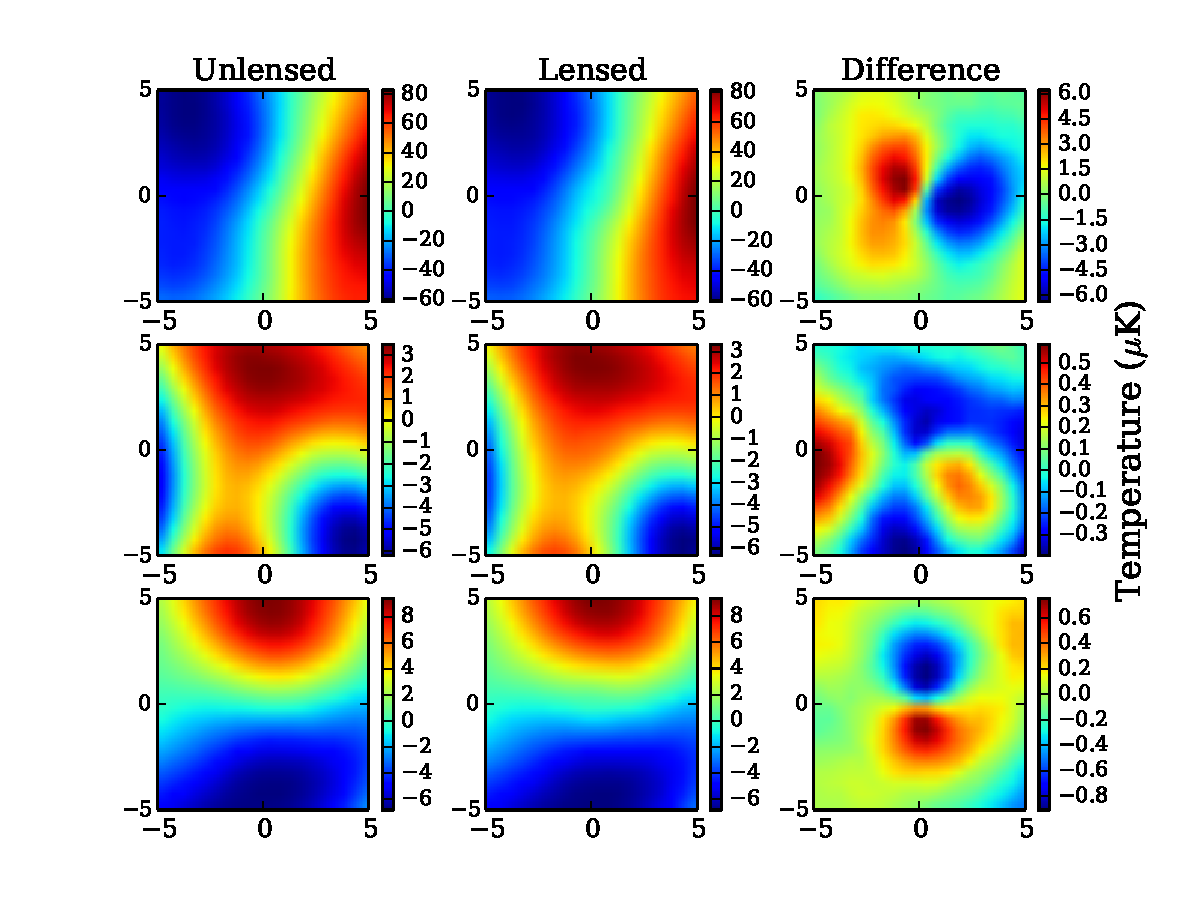
\includegraphics[width=\linewidth, keepaspectratio]{figs/lensing_signal.pdf}
 \caption{Lensing effect on CMB due to a galaxy cluster of mass $5\times 10^{14} M_{\odot}$ .
  On the top panel we show the effect of cluster lensing on CMB temperature field.
  Bottom two panels are for the stokes Q and U parameters.
  The lensing signal for temperature is few $\mu$K and an order of magnitude smaller in polarisation.
  Note that in the above simulation we haven't used either experimental noise or foregrounds. 
 } 
\label{fig:lensing_signal}
\end{center}
\end{figure}

The deflection induced due to lensing is nothing but remapping of the unlensed CMB temperature and polarisation fields based on the gravitational deflection angle. Mathematically lensing is expressed by the following equations
\begin{eqnarray}
T(\hat{n}) = \widetilde{T}(\hat{n} + \vec{\alpha}(\hat{n}))\\
Q(\hat{n}) = \widetilde{Q}(\hat{n} + \vec{\alpha}(\hat{n}))\\
U(\hat{n}) =  \widetilde{U}(\hat{n} + \vec{\alpha}(\hat{n}))
\end{eqnarray}
where $\widetilde{}$ represents unlensed fields, T represents the temperature field, Q and U are the stokes polarisation parameters respectively. 
$\vec{\alpha}(\hat{n})$ is the deflection angle along the $\hat{n}$ direction. 
\\

\subsection*{Deflection angle:}
\label{sec_def_field}
Deflection field depends on the density profile of a galaxy cluster. Here we provide a detailed calculation of deflection field for spherically symmetric Navarro-Frenk-White (NFW) density profile \cite{navarro96}.  Lensing convergence is related to deflection field as %$\nabla \phi (\hat{n})$ and is directly proportional to the mass of the cluster.
%Deflection angle depends on the cluster mass profile. Here we provide the detailed calculation for Navarro-Frenk-White (NFW) density profile \cite{navarro96}. NFW density profile can be characterised by two free parameters $M_{200}$ and concentration parameter $c$ as:
\begin{equation}
 k = \frac{1}{2}\nabla. \vec{\alpha} %#= -\nabla^{2} \phi
\label{eq_kappa}
 \end{equation}
 where $\alpha$ is the deflection angle, $k$ is the lensing convergence profile. % and $\phi$ is the lensing potential.
 For symmetrical density profiles, the lensing convergence is equal to the ratio of surface mass density over the critical surface density of the Universe at the cluster redshift, $k = \frac{\Sigma(x)}{\Sigma_{crit}}$.
The surface mass density or also known as the projected mass density of the halo is obtained by integrating the halo density profile along the line of sight. 
 \begin{equation}
 \Sigma(x) = 2 \int^{\infty}_{0} \rho(r) ds
 \label{eq:surface_density}
 \end{equation}
 where $r$ is the radial distance, $x$ is the corresponding two-dimensional planar distance and $s$ is distance along the line of sight with $s = 0$ being the plane of the cluster.
 The critical surface density of the Universe at cluster redshift is given by
 \begin{equation}
 \Sigma_{crit} = \frac{c^{2}}{4\pi G} \frac{D_{cmb}}{D_{clus}D_{cmb,clus}}
 \end{equation}
 where $D_{cmb}$ is the comoving distance to the epoch of recombination (z= 1100), $D_{clus}$ is the comoving distance to the cluster, and $D_{cmb,clus}$ is the comoving distance between the CMB and the cluster.
 
 Unless otherwise mentioned, we define all the cluster quantities in this chapter with respect to $R_{200}$, which is defined as the radius within which the mean cluster density is 200 times the critical surface density of the Universe at cluster redshift $\rho_{crit}(z)$. By definition $M_{200}$ is given by 
 \begin{equation}
 M_{200} = \int^{R_{200}}_{0}  4\pi x^{2} \rho(x) dx,
 \end{equation}
 $M_{200}$ can also be written as
 \begin{equation}
 M_{200} = \frac{800\pi}{3} R^{3}_{200} \rho_{crit}.
 \end{equation}
 
 The above mathematical equations hold for any spherically symmetric halo. 
 Here we consider a specific case of Navarro Frenk White (NFW) halo density profile.
 In the NFW profile, the density of the dark matter halo as a function of radius is given by:
 \begin{equation}
 \rho(r)= \frac{\delta_{c}\rho_{crit}(z)}{(\frac{r}{R_{s}})(1+\frac{r}{R_{s}})^{2}}
 \end{equation}
 where $\delta_{c}$ is the characteristic over-density, $R_{s}$ is the characteristic scale radius, and $c$ is the dimensionless concentration parameter.
 The dimensionless over-density is given by $\delta_{c} = \rho_{0}/\rho_{crit}(z)$, where $\rho_{0}$ is the cluster central density and  $\rho_{crit}(z)$  is the critical density of the universe at cluster redshift.
 Plugging the above equation in ~\ref{eq:surface_density}, we get the surface density for the NFW halo. 
 By changing the variables of integration to $s=\sqrt{r^{2} - x^{2}}$ and $ds = \frac{rdr}{\sqrt{r^{2} - x^{2}}}$ we obtain:
 \begin{equation}
 \Sigma(x) = 2\delta_{c} \rho_{crit}(z) R^{3}_{s} \int^{\infty}_{x} \frac{1}{r(R_{s} + r)^{2}} \frac{rdr}{\sqrt{r^{2} - x^{2}}}
 \label{eq:sr_den}
 \end{equation}
 The scale radius is related to the concentration parameter as follows:
 \begin{equation}
 c = \frac{R_{200}}{R_{s}},
 \end{equation}
we have set $c = 3.0$ following \cite{bhattacharya13}.
 
 
 Eqn. ~\ref{eq:sr_den} can be solved analytically and the explicit closed-form expression for the NFW case is given by \cite{bartelmann96}. 
 With $\Sigma(x)$ and $\Sigma_{crit}$ in hand we can use Eq. ~\ref{eq_kappa} to get the lensing deflection angle as function of cluster mass and redshift. 
 Unless otherwise mentioned we assume the galaxy clusters follow the NFW profile. However,  the mathematical framework described above can be applied to any halo density profile. 


\section{Maximum Likelihood Estimator}
\label{sec_MLE}
We developed the maximum likelihood estimator to constrain the CMB cluster lensing signal.
 %Gravitational lensing by a galaxy cluster remaps the unlensed CMB field. 
 The unlensed CMB can be assumed to be a Gaussian random field to a very good approximation  \citep{planck14d}.
 CMB-cluster cluster lensing remaps this Gaussian random field based on the deflection angle.
 The remapping can be modeled in the form of a covariance between the data pixels. 
 First, we describe the likelihood estimation in \S~\ref{lkhd_est}, followed by covariance matrix calculation in \S~\ref{sec_covmat}.
\subsection*{Likelihood Estimation}
\label{lkhd_est}
  The likelihood of observing a particular set of pixelized values `$d$' is given by 
  %With the covariance matrix in hand we calculate the likelihood given the data as follows 
  
  \begin{equation}
  -2lnL(d|\Sigma_{lens}) = ln |\Sigma_{lens}| + d^{T} \Sigma^{-1}_{lens} d,
  \end{equation}
 where $\Sigma_{lens}$ is the covariance matrix which acts as a model, $d$ is the pixel values of the observed temperature or polarisation maps.
  %The likelihood function extracts all the lensing information unlike the QE.
  %The pixel values are defined as the variations from the mean CMB temperature (polarisation) (which is zero).
  
  %Since the majority of the lensing singal is within few arcminutes from the cluster center, we carry out the lensing analysis within \smallboxsize\ of the cluster center to simplify and speed up the analysis. 
  %We also checked that by increasing the boxsize to 14\am\ we gain an improvement in a SNR of less than 1\%, however, that the increases the computational complexities. 
  Lensing signal of a single galaxy cluster is too weak to be detected. 
  We stack many clusters to increase SNR (signal to noise ratio) to a reasonable level
  \begin{equation}
  -2ln L(d| \Sigma_{lens})_{tot} = \Sigma^{n}_{i =0} w_{i} [ln |\Sigma_{lens}| + d^{T}_{i} \Sigma^{-1}_{lens}  d]
  \end{equation}
  where n is the total number of clusters in the sample, $w_{i}$ is the weight assigned to the $i^{th}$ cluster.
  Here we assign equal weights to all clusters ($w_{i} = 1$) as we are using simulations and it is not the case while using real data. %While for real data $w_{i}$  which is survey dependent (for example experimental noise etc.,).
%  In this chapter as we are using simulated clusters, we assign uniform weights to all cluster.

%Gravitational lensing by a galaxy cluster remaps the unlensed CMB field inducing non-Gaussianties. 
%This can be encapsulated in the form extra pixel-pixel correlations in the real space. 
%First I describe the calculation of covariance matrix which will act as a model followed by likelihood calculation. %and then I describe the cluster density profile used in modeling. 


\subsection{Covariance matrix calculation}
\label{sec_covmat}

 We calculate the covariance matrix using a set of simulated skies \footnote{more details about simulations are provided in ~\ref{sec_appendix_simulated_skies}}. 
 To simulated the lensed CMB sky, we first generate the large-scale structure lensed CMB power spectra ($C^{TT}_{l}, C^{TE}_{l}, C^{EE}_{l},$ and $C^{BB}_{l}$) form CAMB for the $Planck$ cosmology \citep{planck15-13}.  
 We generate Gaussian random realisations of these power spectra on a \mediumboxsize\ box at 0.25\am\ resolution. 
The generated E and B maps are converted to Q and U maps using:
 \begin{equation}
 E_{l} \pm i B_{l} = - \int d^{2} \hat{n} e^{-i \hat{n}. l}[Q \pm iU] (\hat{n}) e^{\mp 2 i\phi_{l}}  
 \label{eq:coord_trans}
 \end{equation}
 where $\phi_{l}$ is the angle of $l$ as measured from stokes Q axis.
 

 These Gaussian realizations are then lensed by the deflection field (which is obtained as explained in ~\ref{def_field}). 
 We take out the central \smallboxsize\ for covariance matrix calculation.\footnote{lensing maps are generated on \mediumboxsize\ to take into account the large scale gradient on which the lensing signal is linearly dependent}
 The lensing signal is of the order of few arcminutes even for a massive cluster and most of the lensing signal is within a radial distance of  10\am\ from the cluster center.
Increasing the boxsize to 14\am\ $\times$ 14\am\ increases the SNR by $\le$ 1\%, while increasing the computational complexity by multiple folds.

 
 With simulated lensed CMB maps in hand we calculate the covariance matrix as follows
 \begin{eqnarray}
\Sigma_{lens}(M,z) & = & \left<(\textrm{\textbf{G}} - \left<\textrm{\textbf{G}}\right>) (\textrm{\textbf{G}} - \left<\textrm{\textbf{G}}\right>)^{T}\right>\\
  =   \frac{1}{n-1}\sum\limits_{i = 0}^{n} (\textrm{\textbf{G}}_{i} - \left<\textrm{\textbf{G}}\right>) (\textrm{\textbf{G}}_{i} - \left<\textrm{\textbf{G}}\right>)^{T} %(\textrm{\textbf{G}}_{i} - \left<\textrm{\textbf{G}}\right\
%s>)^{T},
\label{eq_lensed_cmb_cov_mass_z}
\end{eqnarray}
 where vector $G_{i}$ is either the polarisation or temperature simulated data for the $i^{th}$ sky realisation and $\langle \rangle$ represents the ensemble average. 
 The number of simulated skies depend on the number of degrees of freedom in the covariance matrix. 
 In our case, the maximum number of degrees of freedom is for the polarisation estimator (concatenated Q/U or E/B maps), for which the covariance matrix is an 800 $\times$ 800 matrix. %the covariance matrix is a 800 $\times$ 800 matrix. 
 Number of simulations scale as twice the number of elements in the covariance matrix. 
  We found that 1,30,000 simulations are sufficient to recover cluster masses without any detectable bias. 
  We then multiply Hartlap correction term $\frac{(n_{sims} -n_{d} -1)}{n_{sims}}$, where $n_{sims}$ is 1,30,000 and $n_{d}$ is the length of the data vector 400(800) for T(QU), to remove any possible bias in $\Sigma^{-1}_{lens}$ due to the limited number of simulations. 
  
 We also use these simulated skies to quantify the effects of statistical and systematic uncertainties.
 There are several astrophysical sources which act as a systematic bias for the CMB-cluster lensing analysis. 
 In this work we consider clusters own SZ effects such as thermal Sunayev-Zel'dovich (tSZ) and kinematic Sunayev-Zel'dovich effects. 
 %tSZ is in explained in detail in the next chapter. 
 Along with these SZ effects, we have also considered sources which are uncorrelated with cluster, such as tSZ effect from other halos, dusty star forming galaxies (DSFGs), and radio galaxies.
 In appendix, we provide more details about the addition of these foregrounds to simulated skies.
 
Here we have used simulations to check the performance of MLE and also to quantify the effect of systematics. 
 Unless otherwise mentioned all the clusters are simulated at a mass of $M_{200} = 2*10^{14} M_{\odot}$ %\footnote{$M_{200}$ is defined as the mass within radius $R_{200}$, which is the radius within which the density is 200 times the critcal density of the Universe at cluster redshift} 
 and at redshift of 0.7.
 For covariance matrix calculation we simulate the clusters at redshift of $0.7$ with mass resolution of $2*10^{12} M_{\odot}$
 Note that such fine gridding might not be computationally feasible for data where the clusters span a wide range of masses and redshifts.
 An optimal solution would be to generate the covariance matrices on coarser grid of mass and redshift and then interpolating it on a finer grid.  
 
 \section{Results}
\label{sec_mle_results}
 In this section, we first validate our pipeline using simulations and we report the expected mass uncertainties for the polarisation and temperature MLE. 
 Then we compare the performance of MLE and QE for ideal simulations by varying only the experimental noise levels and not including any galactic or extra galactic foregrounds. 
 Later, we compare the performance of the estimators in the presence of foregrounds. 
 In this chapter all the results are for a set of 100,000 simulated clusters (expected number of clusters for CMB-S4) each at a mass of $2\times10^{14} M_{\odot}$ and at redshift of 0.7.
\iffalse{
 To obtain the lensing significance, we calculate the ratio of combined likelihood at zero mass to that of maximum likelihood:
 \begin{equation}
 \lambda = \frac{L (M_{200} =0)}{max(L(M_{200}))}
 \end{equation} 
 According the Wilk's theorem, in many cluster limit $\lambda $ follows chi-square statistic with one degree of freedom ($M_{200}$ in our case).
 The detection significance reported in this chapter is equal to $-2 ln (\chi)$
 Similarly, we quote the mass uncertainties by calculating masses at which $-2lnL(M_{est}) + 2 ln L (M_{200})$ is equal to 1, where $M_{est}$ is the best fit mass.
 }\fi
 
 \subsection{Idealised simulations}
 \label{sec_ideal_sims}
 Our baseline simulations include only experimental white noise level.
 These idealised simulations serve two purposes: 
 \begin{itemize}
 \item serve as benchmark to estimate the effect of different systematic and statistical sources of uncertainties on lensing analysis. 
 \item in addition to that, it provides equivalent conditions to allow for a fair comparison between MLE and QE.
\end{itemize}
 To validate the pipeline we simulate 100,000 galaxy clusters each at a mass of $2 \times10^{14} M{\odot}$ and at redshift of $z = 0.7$.
 We add a white noise realisation of rms 1\ukam\ for temperature maps and  rms $\sqrt{2}$\ukam\ to polarisation maps. 
 These simulations are then convolved by a beam of FWHM 1\am\ and then passed through our pipeline.
 The results are shown in the top panel of Fig. ~\ref{lkhd_curve}, the black solid line represents the combined likelihood for temperature MLE estimator and solid (dashed) orange curve is that for the polarisation QU (EB) estimator.% and the dashed orange curve is for EB estimator. 
 We calculate the detection significance as mentioned above and measured a lensing significance of 400$\sigma$ and 110$\sigma$ for temperature and polarisation MLE respectively. 
 Null test results are shown in the bottom panel of Fig. ~\ref{lkhd_curve}, for which we turned off lensing in our pipeline.
 As expected likelihoods for all the three MLE estimators (T, QU, and EB) peak at zero mass.
 
 \begin{figure}[t]
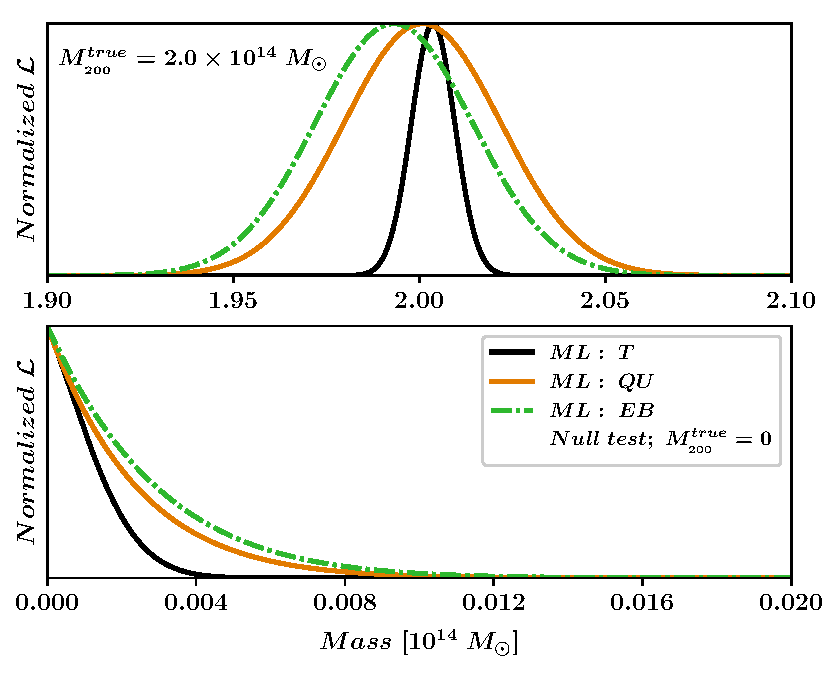
\includegraphics[width=\linewidth, keepaspectratio]{figs/fig0-eps-converted-to.pdf}
 \caption{In the top panel we show the combined likelihood of 100,000 clusters each at redshift of 0.7 and at mass of $2\times 10^{14} M_{\odot}$ for temperature and polarisation MLE estimators. The difference between QU and EB estimator isn't statistically significant. In the bottom panel we show the results of null test and as expected the likelihood peaks at zero for all three estimators}
\label{lkhd_curve}
 \end{figure}
 
 In the left panel of Fig.~\ref{fig_performance}, we compare the performances of the three MLE estimators and the temperature QE estimator as a function of experimental noise levels. 
 %Note that, no galactic or extra galactic foregrounds are added. 
 %All the fractional mass uncertainties are stated for 100,000 clusters each at a mass of $2\times 10^{14} M_{\odot}$ and at a redshift of 0.7.
 It is evident from the Fig.~\ref{fig_performance} that in the absence of foregrounds, temperature estimator outperforms polarisation above noise-level of 0.075 \ukam.
 So even for future experiments temperature estimator has to be the primary channel from pure SNR perspective.
 Only below the noise-level of  0.075 \ukam do polarisation estimator begin to be competitive with temperature.
 The relative performance of the temperature and the polarisation estimators can be understood as:
 \begin{itemize}
 \item lensing signal scales the amplitude of the background gradient which is $\sim$10$\times$ brighter in temperature, but
 \item as the experimental noise levels drop, the background CMB acts as an additional source of noise for the temperature estimator.
 \end{itemize}
 %As pointed out earlier, the lensing signal is directly proportional to the background CMB gradient, gradient in polarisation is 10$\times$ smaller than that of temperature as shown in ~\ref{fig:lensing_signal}. However, below noise-level of 0.075\ukam the CMB temperature background gradient acts as a source of noise. 
 
 Orange squares and green circles in Fig. ~\ref{fig_performance} represent MLEs using polarisation QU and EB maps respectively. 
 As expected, there is no significant differences between their performance from a theoretical standpoint. 
 The apparent difference at higher experimental noise levels is not statistically significant.
 However, using QU maps simplifies the analysis as these modes are directly measured by the experiment and doesn't involve co-ordinate transformation. %~\ref{eq:coord_trans}. %In this chapter, I have considered only $QU_{MLE}$ polarisation estimator.
 
  
 Lastly, we compare the performance of temperature MLE (solid black triangles) and QE (orange solid squares) in Fig. ~\ref{fig_performance}. 
 QE is a first order approximation of MLE (as we will see in ~\ref{ch:mqe}).
 %While both temperature MLE and QE perform equally well at higher noise levels, MLE has clear advantage over QE at low noise levels.
 At higher noise levels (low SNRs) the effect of higher order terms are negligible resulting in no difference between the performance of MLE and QE estimators.
 However, at low noise levels (high SNRs) MLE outperforms QE. We find that MLEs performance improves by a factor of 2 at noise level of 0.1\ukam for our fiducial cluster sample. 
 The performance of QE can be improved by using an iterative version as shown in \cite{yoo08}.
  %Though not shown here, there is no difference between polarisation MLE and QE for the range of the experimental noise levels we have considered.
  %This is not surprising as polarisation lensing SNR is low for all the considered noise levels.
 %The effect of higher order terms can be recovered using an iterative version of QE as shown in \cite{yoo08}.
 %We find that MLEs performance is improves by a factor of 2 at noise level of 0.1\ukam  for our fiducial sample of 100,000 clusters each at  $M_{200} = 2 \times 10^{14}$ \msolar and redshift of 0.7. 
  
Both MLE and QE estimators share a common difficulty in regards with the assumed cluster density profile.
This dependence shows up in different places in each estimator:
 \begin{itemize}
 \item In MLE as explained in ~\ref{sec_MLE} we fit the lensed CMB pixel covariance templates to the observed data pixel covariance. The lensed CMB pixel covariance templates are obtained by assuming a cluster density profile. 
 \item QE works by exploiting the correlation between the background CMB gradient and lensing dipole to obtain lensing convergence profile. 
 We fit models to these lensing convergence profile to extract the mass of the cluster.
 
 \end{itemize}
While MLE outperforms QE at low experimental noise level, QE can be modified to make it robust to the major foreground in lensing analysis as we will see in next chapter (~\ref{ch:mqe}).
 \begin{figure}[t]
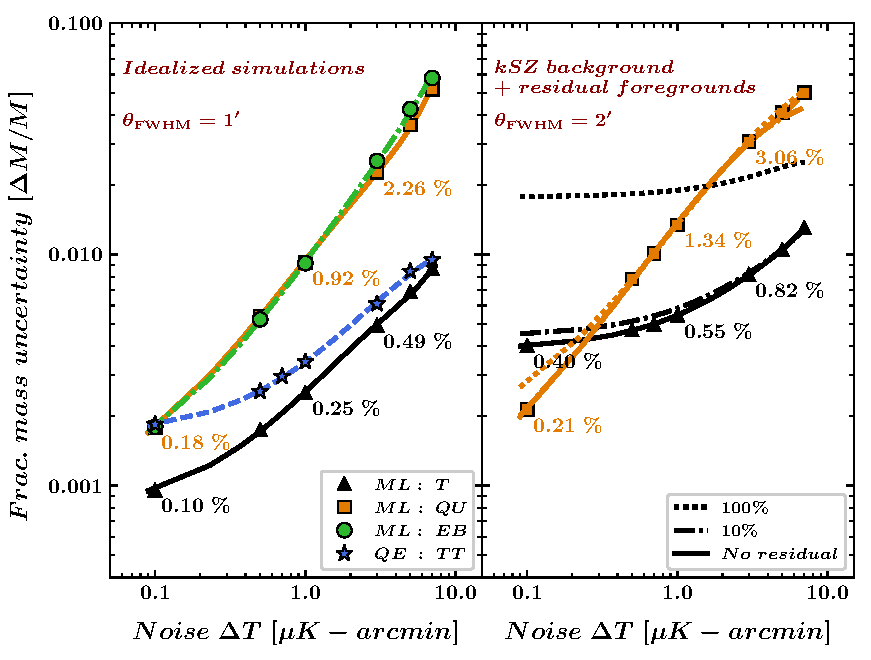
\includegraphics[]{figs/fig1-eps-converted-to.pdf}
 \caption{In the left we show the performance of different estimators for idealised simulations as function of experimental noise levels. We consider the effects of various foregrounds on the estimators in the right panel. All the curves are for a set of 100,000 clusters each at mass of $2\times 10^{14} M_{\odot}$ and at redshift of 0.7.}
 \label{fig_performance}
 \end{figure}
   
   \subsection{Effects of extragalactic foregrounds on lensing analysis}
   In this section, we look into the effects of extragalactic foregrounds on CMB-cluster lensing analysis. While galactic foregrounds also affect the CMB-cluster lensing analysis, we can exploit their frequency dependence to suppress galactic contamination. Here we consider the effect of extra galactic foregrounds on mass uncertainties. Some of these foregrounds such as clusters own SZ effect etc., also bias the analysis which will be reported in the next section (~\ref{sys_bias}). The level of foregrounds is much higher in temperature than in polarisation channel, thus the effect of foregrounds is higher in temperature estimator than polarisation. We consider the impact of tSZ, kSZ, radio galaxies and dusty galaxies on lensing analysis.
   
   The impact of foregrounds on the fractional mass uncertainty of lensing estimators as function of experimental noise level is shown in Fig. ~\ref{fig_performance}. 
   As expected foregrounds have negligible effects on the polarisation channel (orange squares) due to their low level of polarisation.
   For the temperature estimator the extragalactic foregrounds set an effective noise level of 5\ukam if not cleaned, this results in plateauing at 1.8\% in mass uncertainty (black dotted line). 
   Without any foreground cleaning polarisation QU estimator outperforms the temperature channel at 1.5 \ukam noise level.
 However, we can exploit the frequency dependence of various extragalactic foregrounds to reduce their effect.
 While combining multiple frequency channels we assume that the beam size is 1\am\ FWHM Gaussian irrespective of the frequency channel to simplify the analysis \footnote{ this may not be a very good assumption, but here we just want to build an intuition for future surveys.}. 
Using different spectral dependence of background CMB and tSZ we can completely eliminate the tSZ power.
While tSZ can be eliminated, kSZ has the same spectral dependence as that of the CMB and cannot be eliminated using linear combination of different frequency channels.
 
 
 Furthermore we assume that the frequency cleaning will behind some radio and dusty galaxy power \footnote{note that in all the curves we have assumed 100\% kSZ power and 0\% tSZ power}. 
 The black solid line in Fig. ~\ref{fig_performance} correspond to 100\% removal of radio and dusty galaxy power. 
 The dot-dashed (dashed) line corresponds to 90\% (0\%) removal of radio and dusty galaxy power. 
 % represent the performance of temperature estimator with 100\% kSZ signal but no tSZ, radio or dusty galaxy signals.
%The dot-dashed (dashed) line corresponds to 100\% of kSZ, no tSZ and 100\%(10\%) of radio and dusty galaxy power.
 %The dashed line corresponds to 10 \% of radio and dusty galaxy power, 100\% of kSZ power and no tSZ power. 
 With 90\% cleaning of foreground (dashed black curve), temperature estimator becomes the main channel for estimating lensing signal even for future surveys \citep{cmbs4-sb1}.
  There is only a fractional improvement in the performance above 90\% of cleaning. 
  It is important to note here that foreground cleaning enlarges the beam which if taken into account will further degrade the mass uncertainties.
  
  To summarize, the extragalactic foregrounds have almost no effect on the performance of polarisation estimators. 
  On the other hand, temperature estimators will have effective noise floor of 5\ukam\ if the foregrounds aren't taken into account. 
  %As we will see in next in addition to increasing final mass uncertainties, some of these foregrounds will also acts sources of systematic bias.
  
  \section{Systematic bias checks}
  \label{sys_bias}
  From Fig ~\ref{fig_performance}, it is evident that we will achieve unprecedented statistical uncertainties for future low noise surveys. 
  However, in order to fully utilise this statistical power, we need to account for all the systematic biases involved in lensing analysis. %to claim our sub-percent mass measurements.
    In this section, we quantify various sources of systematics that could bias our final results.
    We examine the following sources:
    \begin{itemize}
    \item cluster center - for example, typical offset between SZ and X-ray centroid is 0.5 \am\ \citep{linden14}
    \item cluster density profile - the assumed NFW profile may not match the true density profile
    \item lensing by other halos - in addition to the galaxy cluster CMB is also lensed by other halos along the line of sight 
    \item redshift - misestimation of cluster redshit
    \item cluster's tSZ effect
    \item cluster's kSZ effect
    \item dusty galaxies
    \end{itemize}
    The last three sources have negligible effect on the polarisation estimators as they are partially polarised. 
    Note that all these sources may effect polarisation and temperature estimators to different extents as the angular scales are weighed differently in both estimators. %due to the differences in mode weighing between estimators.
     
 The baseline simulations for bias calculations include 1\am\ FWHM Gaussian beam, experimental noise level of 1\ukam in temperature (which corresponds to a noise level of $\sqrt{2}$\ukam in polarisation) and no foregrounds unless otherwise stated.
  While the precise amount of bias depends on experimental beam size, noise-level, and foregrounds as they define the weighing of different angular scales of MLE, here we roughly quantify the magnitude of bias and give a direction to pursue future work in CMB-cluster lensing to reduce the systematic uncertainties. 
   We report the systematic bias for a sample of 1,000,000 clusters each at a mass of $2 \times 10^{14}  M_{\odot}$ and at redshift of 0.7 (except for redshift uncertainty case). The bias is calculated as follows:
   \begin{equation}
   b = \frac{M_{bias}}{M_{true}} - 1.
   \end{equation}
   where $M_{bias}$ is the final recovered mass when the bias source is included in the lensing analysis and $M_{true}$ is the input mass. 
   Error on the bias is obtained by calculating the scatter in 100 subsamples.
   
   We report bias for all the sources considered in Table ~\ref{`}. 
 Other than errors in redshift, all other sources of bias should be considered carefully to achieve sub-percent uncertainty as claimed for future CMB surveys \citep{cmbs4-sb1}. 
 %Here we have not considered survey specific systematics such as false detections, selection function, and projection effects or some form of bias in weighing the clusters.
 \begin {table}[ht]
%\caption{Systematic bias in the reconstructed lensing mass}
\centering
%\resizebox{0.5\textwidth}{!}{
\begin{tabular}{| l | c  | c | c | c |}
    \hline
    \multirow{2}{*}{Bias source} & \multicolumn{4}{c|}{Bias \% at $\Delta T = 1.0\ \ukarcmin$}\\
    \cline{2-5}
    & \multicolumn{2}{c|}{Temperature $T_{\rm ML}$} & \multicolumn{2}{c|}{Polarization $QU_{\rm ML}$} \\%\hline
    \cline{2-5}
     & \% bias& error & \% bias & error \\\hline
    tSZ cleaning (1\% residual signal) & -6.3 & 0.50 & 0 & - \\\hline
    kSZ fitting (20\% uncertainty) & -7.3  & 0.31 & 0 & - \\\hline

    DG in the cluster & -4.5 & 1.70 & -1.3 & 1.20\\\hline
    \hline
    Redshift uncertainty & {\ }0.2 & \multirow{2}{*}{0.25} & -0.3 & \multirow{2}{*}{0.90} \\%\hline
    \cline{1-2}\cline{4-4}
    Cluster positions & -7.5 & & -1.5 & \\\hline
    \hline
   Presence of undetectable haloes & 2.5 & 0.25  &6.3 &0.92\\
    \hline\hline
    \multicolumn{5}{|l|}{Uncertainties in cluster mass profile}\\\hline
   ~~~$\kappa_{\rm NFW} + \kappa_{sub}$ & {\ }3.1 & \multirow{4}{*}{0.25} & -0.6 & \multirow{4}{*}{0.92}\\%\hline
    \cline{1-2}\cline{4-4}
    ~~~$\kappa_{Einasto}$ & -2.4 & & -2.5 &\\%\hline
    \cline{1-2}\cline{4-4}
    ~~~$\kappa_{\rm NFW}^{^{mod}}$ & {\ }2.2  & & {\ }0.6 & \\\hline

 \end{tabular}
\vspace*{2mm}
%}
%\tablecomments{
\caption{The percentage mass biases from various systematic uncertainties. A positive (negative) number means the recovered mass is over- (under-)estimated. The first three lines reflect the expected biases from astrophysical foregrounds; these are serious for the temperature estimator, but not the polarization estimator. The next two lines deal with uncertainties in where the cluster is located (whether in redshift or on the sky); these are likely to be manageable for both estimators. The last four lines relate to uncertainties in how the mass is distributed, whether due to projection effects from nearby, lower-mass haloes, or due to uncertainties in the average mass profile for galaxy clusters. These questions about the mass distribution are a concern for both temperature and polarization. }
%\caption{Systematic bias in the reconstructed lensing mass}
\label{tab_sys_bias}
\vspace*{2mm}
\end{table}
 \subsection{Halos along the line of sight}
 In addition to galaxy cluster, the lensing signal also depends on other halos present along the line of sight as well as the correlated halos. 
 If the effect due to these halos isn't taken into account then the final results will be biased high. 
 This is particularly a major concern for low mass haloes as they won't be detected by the survey.
 To quantify the effect of this bias we use \cite{flender16} simulations. 
 The \cite{flender16} simulation is an N-body cosmological simulation with 17 million objects.
  For each cluster we randomly select a halo within a mass range of  $M_{200} \in$ [1.8, 2.2] $10^{14} M_{\odot}$ and redshift range of [0.6,0.8].
We simulate the CMB maps as explained earlier, however, instead of lensing the CMB with just the cluster convergence profile we lens it with all the convergence profiles which are within the 50\am\ from the cluster center. 
Analysis proceeds normally after this - these lensed CMB maps are convolved by Gaussian beam after which specified white experimental noise is added. 
As expected both polarisation and temperature estimators are biased high : 2.5 $\pm$ 0.3\% for temperature MLE and 6.3 $\pm$ 1.1\% for polarisation QU estimator. We can reduce the bias by taking two halo term into account, however, that will include more nuisance parameters increasing the statistical uncertainty of the final results. 


Along with the correlated halos and halos along the line of sight, large scale filaments also bias the lensing analysis which is not considered here. 
Galaxy clusters are not isolated objects, they are generally found in large scale filaments. 
Also, clusters with ellipticity along the line of sight have higher tSZ increasing the probability of their detection in tSZ surveys. 
The scope of finding the bias due to the large filaments and selection function is outside the scope of this thesis. 
Its worth noting that in order to fully realise the potential of future surveys in obtaining sub-percent mass uncertainties, we need to work bias due to large scale filaments and cluster ellipticity.
Accurate and reliable simulations of structure formation on large volumes are needed in order to handle this source of systematic error at the sub-percent level.

\subsection{Cluster mass profiles}
\label{sec_den_profiles}
As mentioned the lensing estimators assume a density profile which will certainly differ from the true cluster profile. 
Any difference between the assumed mass profile and true cluster profile will bias the final results.
In this work we assume the clusters to follow an NFW profile. 
However, studies have shown that for massive clusters the density profile deviates significantly from NFW at radius $r \ge 0.5 \times R_{200}$ \citep{diemer14}. 
It is unknown whether these deviations will be larger or smaller for lower mass clusters.
Also a recent study has shown that for analysis involving stacked halos Einasto profile \citep{einasto89} provides a better estimate \citep{child18}.
Here we consider three density profiles in order to estimate the bias.
\begin{itemize}
\item A modified version of the NFW profile which drops off more rapidly with radius
\begin{eqnarray}
\kappa_{\rm NFW}^{mod}(x) =
\begin{cases}
    \kappa_{\rm NFW} &; x \le 0.75\theta_{_{200}}\\
    \kappa_{\rm NFW} \times m(i,j)&; 0.75\theta_{_{200}} < x \le 1.5\theta_{_{200}}\\
    0 &; otherwise
\label{eq_kappa_mod}
\end{cases}
\end{eqnarray}
where $m(i,j)$ is a Hanning two-dimensional (2D) apodization kernel.
We create the 2D apodization kernel as $m(i,j) = m(i) \times m(j)$ with $m(i) = \frac{1}{2} \left[ 1 - cos\left(\frac{2\pi  (i-n/2) }{n} \right)\right]$, where i and j are pixel indices in the $n \times n$ map.
\item A change to the cuspiness of cluster core in the NFW profile following \citet{king01} 
\begin{eqnarray}
\kappa_{\rm NFW}^{sub}(x)  & =  &
\begin{cases}
    \kappa_{\rm NFW}\ + \sum\limits_{i=1}^{3} \kappa_{sub}^{i}&; x \le 1'\\
    \kappa_{\rm NFW} &; otherwise;
\label{eq_kappa_sub}
\end{cases}
\end{eqnarray}
\item The Einasto profile \citep{einasto89}
\begin{eqnarray}
\rho(r)_{_{Ein}} & = &  \rho_{_{0}}\ exp\left( - \frac{2}{\alpha} \left[\left(\frac{r}{R_s} \right)^{\alpha} - 1\right]\right)
\label{eq_einasto_density}
\end{eqnarray}
with the shape parameter $\alpha = 0.18$ \citep{ludlow13}. The Einasto convergence profile is obtained by inserting this into Eq.(\ref{eq:surface_density}).
\end{itemize}
 
 In each of the three cases we lens CMB by the assumed cluster profile, however, we use NFW profile to calculate our model.
 Assuming the wrong cluster profile biases the results from -2.5\% to 3.8\% as shown in Table ~\ref{tab_sys_bias}. 
 A similar study was done on optical weak-lensing analysis by \citet{sereno16} who used NFW profile in the model and Einasto profile in the simulated data; \citet{sereno16} found a bias of -2 to 7 \% depending on the cluster mass. This level of bias is larger than the statistical mass uncertainties expected for the proposed future experiment \citep{cmbs4-sb1}, and a significant challenge for upcoming experiments.
More work will be required to accurately measure the cluster mass profiles as a function of radius if we are to achieve the full potential of galaxy cluster cosmology. 

\subsection{Cluster miscentering}

Any difference between the true cluster center and the model will result in a bias.
 Misestimation of the cluster center even by a small amount results in underestimation of cluster mass as we lose some of the lensing signal.
To quantify the effect of miscentering, we draw an offset from a normal distribution N(0, $\sigma^{2}$) and lens the CMB with offseted clusters to obtain simulated data, however, model doesn't take the offset into account.
Fig. ~\ref{fig_sys_bias_cluster_offsets} shows the bias in the final results as a function of offset for both temperature (orange squares) and polaristion estimators (black triangles).
As expected the bias increases with the rms offset, `$\sigma$'.
The bias in temperature estimator is smaller than polarisation is because the temperature estimator draws more information from smaller angular scales than the polarisation estimator. Note that here we haven't considered foregrounds, considering foregrounds would decrease the weight of smaller angular scales. For survey with higher experimental noise, larger beams and foregrounds the bias due to miscentering will be smaller.

 
The typical offset between the SZ-centroid and the X-ray or brightest central galaxy (BCG) is of the order of 0.5\am\  \citep{linden14,song12b,sereno16}.
For 0.5\am\ offset the mass is underestimated by 7.5 $\pm$ 0.3\% for temperature estimator and 1.5 $\pm$ 1.3 \% for polarisation estimator. 
For a given constraint on the offset, a correction could be easily applied to eliminate the bias, however, that will result in a slight decrease of SNR.
Neglecting the foreground power, one would need to know the rms offset $\sigma$ by 2\% (8\%) in order to achieve sub-percent uncertainty for the temperature (polarisation) MLE.
However, adding foregrounds will reduce the weight of the information from smaller angular scales and lessen the requirement of how well the positional uncertainty must be known.
\begin{figure}[t]
\centering
%\hspace{-2mm}                                                                                                                               
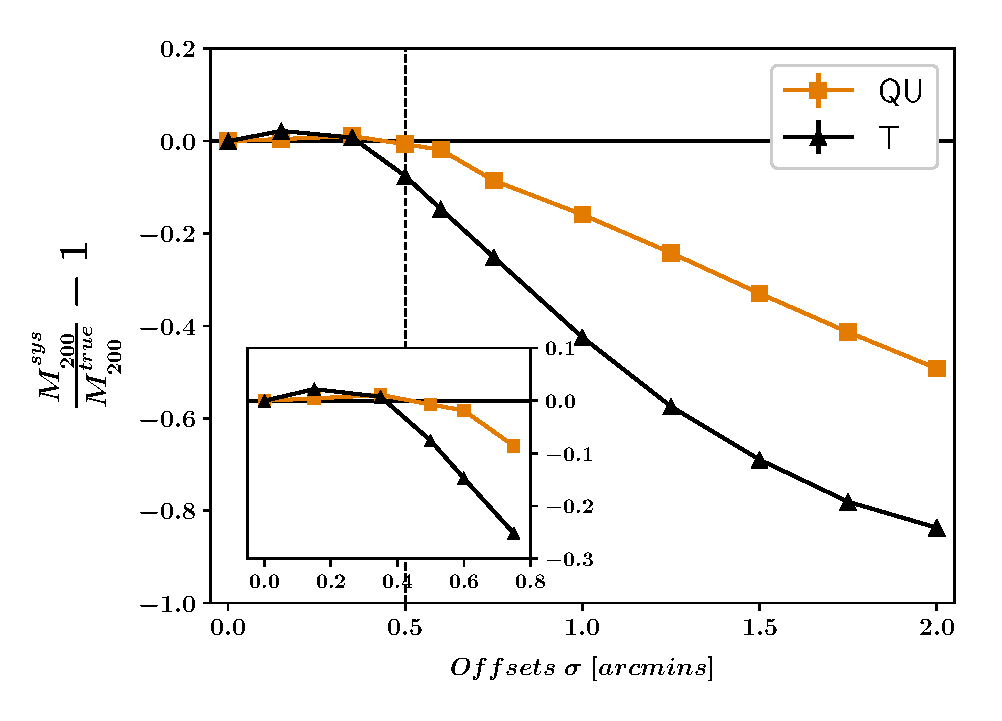
\includegraphics[width=0.85\textwidth, height=0.65\textwidth,clip=]{figs/fig2_v2.eps}
\caption{The positional offset between the assumed and true cluster centroid will bias the estimate low  for $T_{\rm ML}$ (b\
lack triangles) and $QU_{\rm ML}$ (orange squares) estimators. The typical positional offset of $0.5'$ \citep{linden14,song12b,sereno16} is marked with the vertical dashed line. The error bars are derived using estimates gathered by repeating the test 100 times.}
\label{fig_sys_bias_cluster_offsets}
\vspace*{2mm}
\end{figure}


 \subsection{Bias due to redshift uncertainty}
%CMB-cluster lensing can be used to calibrate the mass scaling relations of SZ surveys (SPT-3G, AdVACT, Simons Observatory etc.,), optical surveys (LSST, DES etc.,), and X-ray surveys (eRosita etc.,). 
Upcoming surveys such as \citep{benson14,so18, cmbs4-sb1} are expected to return tens to hundreds of thousands of clusters. 
 At these numbers obtaining spectroscopic redshift for each cluster will be infeasible.  
Instead we likely rely on red sequence redshifts up to a redshift $\sim$ 1.5 and lower limits on the redshift for clusters at even higher redshifts. 
The current state of the art for red sequence redshifts can be seen in the  DES \texttt{redMaPPer} catalog, where the \emph{photo-z} errors are $\sigma_{z} = 0.01 (1+z)$ for $z \le 0.7$ and $\sigma_{z} = 0.02 (1+z)$ for $z \sim 0.9$ \citep{rykoff16}. We examined the effect of the expected redshift uncertainty by considering a redshift scatter for individual clusters. We conservatively take the redshift errors to be
\begin{equation}\nonumber
\sigma_z = \left\{
\begin{array}{l}
    0.02 (1+z);  ~~z < 1 \\
    0.06 (1+z);  ~~z > 1
  \end{array}\right.
\end{equation}

We create mock lensed CMB maps for four sets of redshifts redshifts $z\in[0.5, 1, 1.5, 2]$. While constructing the pixel-pixel covariance matrix we use the `measured' redshift, $z + \sigma_{z}$, for each cluster.                                                                        
The resulting bias is listed in Table~\ref{tab_sys_bias}. We do not detect a mass bias at any redshift. 
 
\subsection{Bias due to the kinematic SZ signal}
\label{sec_ksz_bias}
CMB photons get doppler shifted due to the relative motion of the galaxy cluster with respect to the CMB rest frame, this is known as kinematic Sunyaev-Zel'dovich effect (kSZ) \citep{sunyaev72}.
While the kSZ effect is an order magnitude smaller than the tSZ, unlike tSZ effect, the kSZ effect has the same spectral dependence as that of CMB. 
We cannot combine multiple frequency channels to eliminate the kSZ effect. 
However, we can use polarisation information as the kSZ effect is largely unpolarised  \citep{sazonov99}.

To quantify the kSZ bias on the temperature estimators we consider the publicly available kSZ maps and halo catalog from \citet{flender16} simulations.
These are full sky simulations is in the healpix \citep{gorski05} pixelisation scheme with nside of 8192 correpsponding to 0.42 arcminute resolution.
Within the mass range of $M_{200} \in [1.8 \times 10^{14},2.2 \times 10^{14}]$ $M_{\odot}$ and $z$ $\in$ [0.6,0.8] the catalog has 20,000 halos. 
For each cluster in the simulated data we randomly pick clusters from this set of 20,000 halos. For each cluster we take a 50\am\ $\times$ 50\am\ cutout centered around the halo, smooth it with experimental Gaussian beam of FWHM = 1\am\ and add it to the lensed cluster cutout. 

Final results are significantly biased low at 41\% level if the kSZ effect is not taken into account while modeling the pixel-pixel covariance matrix. We get similarly large levels of bias when we use an analytical model for the cluster kSZ signal instead of extracting them from N-body simulations. Modelling the optical depth of the clusters using the \citet{battaglia16b} profile and drawing the cluster velocities from a normal distribution $N(0, \sigma^{2})$ with scatter $\sigma = 350\ km/s$, we obtained a 32\% bias in the recovered lensing mass.
  
 If we take the effect of kSZ while modeling the pixel-pixel covariance matrix then as expected we eliminate the bias. 
 However, we don't exactly know the kSZ effect of a single cluster. According to current estimates the uncertainty in kSZ prediction is 20\% for a single galaxy cluster. 
 The reason for the uncertainty is the complex cluster baryonic physics which is not very well understood. 
 To determine the bias that would result due to the uncertainty in kSZ effect, we test including 20\% uncertainty in the kSZ modeling for the pixel-pixel covariance matrix. 
 This results in a low bias of 7.5 $\pm $ 0.4 \%, the stated bias can either be low or high depending on underestimation or overestimation of kSZ.
 Interpolating linearly between the kSZ uncertainty and the bias, we find that 2-3\% uncertainty in kSZ would lead to sub-percent systematic uncertainty. 
 Given the current uncertainties in kSZ estimation, it acts as a serious obstacle in using temperature information of CMB-cluster lensing for future CMB surveys. 
 
 \subsection{Thermal Sunayev-Zel'dovich effect}
 \label{tSZ_effect_bias}
Here we give a brief review of thermal Sunayev-Zel'dovich (tSZ) effect and is explained in detail in the next chapter.
CMB photons while passing through galaxy cluster are inverse compton scattered of high energetic electrons present in the cluster's hot intra cluster medium.
This results in excess of photons at higher frequency and deficit of photons at lower frequency, this is known as tSZ effect.
tSZ effect is an order of magnitude greater than lensing signal and will induce significant statistical and systematic uncertainties if not taken into account.
In the next two chapters we discuss in detail about the methods through which we eliminate the tSZ bias in QE estimator.
Here, we quantify the tSZ bias in the MLE and discuss the methods that can be used to reduce the bias.
We consider two different approaches:
\begin{itemize}
\item use frequency channels to eliminate the tSZ
\item model the tSZ effect in the pixel-pixel covariance matrix
\end{itemize}
Either approaches has the potential to completely eliminate the bias, however, due to imperfect knowledge of the instrument calibration or the tSZ profile may leave residual bias. 


To evaluate the performance of each approach,  we use Compton $y$ maps produced on a $5^{\circ} \times 5^{\circ}$ box at resolution $2.'5$ from the smoothed-particle hydrodynamics (SPH) simulations of  \citet{mccarthy13}.
Neglecting relativistic corrections, we convert the Compton $y$ maps into temperature at an observing frequency according to:
\begin{eqnarray}
\Delta T = y T_{\rm CMB} \left[x \left(\frac{e^{x/2} + e^{-x/2}}{e^{x/2} - e^{-x/2}}  \right)\right]
\end{eqnarray} where $x = \frac{h\nu}{k_{\rm B}T_{\rm CMB}}$, $\nu$ is the frequency in GHz, $T_{\rm CMB} = 2.73\ K$, $k$ is the Boltzmann constant, and $h$ is the Planck constant.

\subsubsection{tSZ frequency cleaning}
\label{subsec:tszbias}
 Using the spectral dependence of tSZ we can eliminate it by using CMB maps observed at different frequency channels.
 In this chapter we assume the CMB is observed at 90 GHz and 150 GHz channels with Gaussian beam of FWHM 1.7\am\ and 1\am\ respectively.
 %The tSZ amplitude at 90 GHz is 1.67 times that of 150 GHz.
Using a linear combination 90 and 150 GHz channels, we obtain tSZ free map as follows:
 \begin{equation}
\widetilde{T}(\hat{\textbf{n}})  =  \frac{f\widetilde{T}_{{150}}(\hat{\textbf{n}}) - T_{{90}}(\hat{\textbf{n}})}{f-1}\\
%\end{equation}
%\begin{equation}
%\widetilde{T}_{{150}}(\hat{\textbf{n}})  =  T(\hat{\textbf{n}})_{{150}} \ast \frac{B_{{90}}(\hat{\textbf{n}})}{B_{{150}}(\hat{\textbf{n}})},
%\label{eq_smooth}
\end{equation}
where
 \begin{equation}
 \widetilde{T}_{{150}}(\hat{\textbf{n}})  =  T(\hat{\textbf{n}})_{{150}} \ast \frac{B_{{90}}(\hat{\textbf{n}})}{B_{{150}}(\hat{\textbf{n}})}
 \label{eq_smooth}
 \end{equation}
 is the 150 GHz map convolved by the ratio of the 90 and 150 GHz beam functions. 
 The factor `f' is ratio of tSZ amplitude in 90 and 150 GHz. %It is important to note that 150 GHz has been smoothed with 90 GHz beam using Eqn. ~\ref{eq_smooth} before subtracting out tSZ.
 
We also assume that the experimental noise level in both 90 and 150 GHz channels is 1 \ukam. 
  Under these assumptions using a tSZ free map will eliminate the bias (b = 0.0 $\pm$ 0.7\%). However, it degrades the final SNR by a factor of three as shown in \citet{baxter15}.
  In practice, it is unlikely to obtain a precise value of factor `f' due the uncertainties in frequency band widths or errors in relative calibration of frequency bands.
  To evaluate the bias in the final results due to the uncertainties in the factor `f', we use simulations. 
  We assume an uncertainty of 1\% in f, which is overly conservative for future CMB surveys but comparable to that of current surveys.
 An error in f will result in leakage of tSZ in the final tSZ free maps and will bias the results.
 For 1\% uncertainty in `f' we find the final results to be biased low by -6.3 $\pm$ 0.7 percent. 
 The bias can shift depending on whether the SZ leakage is over estimated or under estimated.
  
tSZ has no power at 217 GHz and one might consider of using 217 GHz frequency channel instead of creating tSZ free maps. 
However, the power of dusty galaxies increase significantly with frequency.
So, the foreground power in 217 GHz channel is much more than 90 or 150 GHz channels. 
In addition to that, we should also take into account the contamination due to the correlation between the tSZ and cosmic infrared background due to these dusty galaxies.
 Current estimates find the correlation co-efficient to be $0.113^{+0.057}_{-0.054}$ \citep{george15}; estimating the tSZ-CIB signal at 220 GHz would yeild a signal nearly three quarters of the tSZ signal at 150 GHz. 
 In order to use 217 GHz channel, more work needs to be done in constraining the tSZ-CIB correlation.
 
 \subsubsection{tSZ fitting}
 Another way to tackle tSZ signal is by modeling it in pixel-pixel covariance matrix.
 We calculate the expected tSZ contribution using SPH simulations from \citet{mccarthy13}.
As one expects, with perfect knowledge of tSZ we get a bias consistent with zero (b = $1.0 \pm 0.6\%$).
However, similar to tSZ frequency cleaning the bias increases quickly if the tSZ contribution is mis-estimated.
Misestimating the tSZ signal by 1\% leads to significant (order 6\%) shifting the recovered mass.
Given that the current uncertainties in modeling the tSZ signal from galaxy clusters are at least an order of magnitude larger, it will be extremely challenging to achieve the sub-percent precision necessary to make this approach viable.
%Another way is to subtract tSZ model from the 150 GHz channel.
 %While this method doesn't degrade the SNR unlike the frequency cleaning, however, imperfect knowledge in theoretical modeling will result in a bias.
 
 
 
 \subsection{Dusty galaxies in the cluster and other foregrounds}
\label{sec_DG_sys_bias}


Galaxy clusters are known to host overdensities of dusty galaxies, with several papers measuring the resulting tSZ-CIB correlation \citep{dunkley13, george15, planck16tsz-cib}.
We describe our modeling of these DG overdensities\footnote{For implementation reasons, in this section, we include all foregrounds mentioned in the Appendix \ref{sec_appendix_simulated_skies}, even ones that are not correlated with the cluster itself, such as radio galaxies.} in the Appendix \ref{sec_appendix_extragal}.
If ignored, the tSZ-CIB correlation may substantially bias the recovered masses from temperature estimators, especially at higher frequencies.
The emission from dusty galaxies rises sharply with frequency, by an order of magnitude in $\mu K^2_{\rm CMB}$ from 90 to 150\,GHz and again from 150 to 220\,GHz.
Polarization estimators (at least at 150\,GHz and lower frequencies) are essentially unaffected due to the lower polarization fraction  of dusty galaxies (expected to be less than 4\% \citep{manzotti17,seiffert07}).
The tSZ-CIB correlated power could be handled analogously to either the tSZ fitting or cleaning approaches in \S\ref{subsec:tszbias}.
However, a multi-frequency cleaning scheme will be less effective than for the tSZ effect since the spectral dependence of thermal dust emission varies between individual galaxies.
Here we look only at bias for the fitting approach where the pixel-pixel covariance due to the clustered dusty galaxies is folded into the likelihood.
The recovered mass is somewhat low: $b=4.5 \pm 1.7\%$.
The existence of a bias (higher than $2\sigma$) is slightly surprising since one would expect zero bias in the perfect information limit, and the significance is low enough that it may be a statistical fluke.
The dramatic increase in the uncertainty -- from 0.25\% to 1.7\% -- reflects the plateauing of the dotted line in right panel of Fig.~\ref{fig_performance}.
Unsubtracted foreground power effectively sets a lower bound on the instrumental noise.


\begin{figure}[ht]
\centering
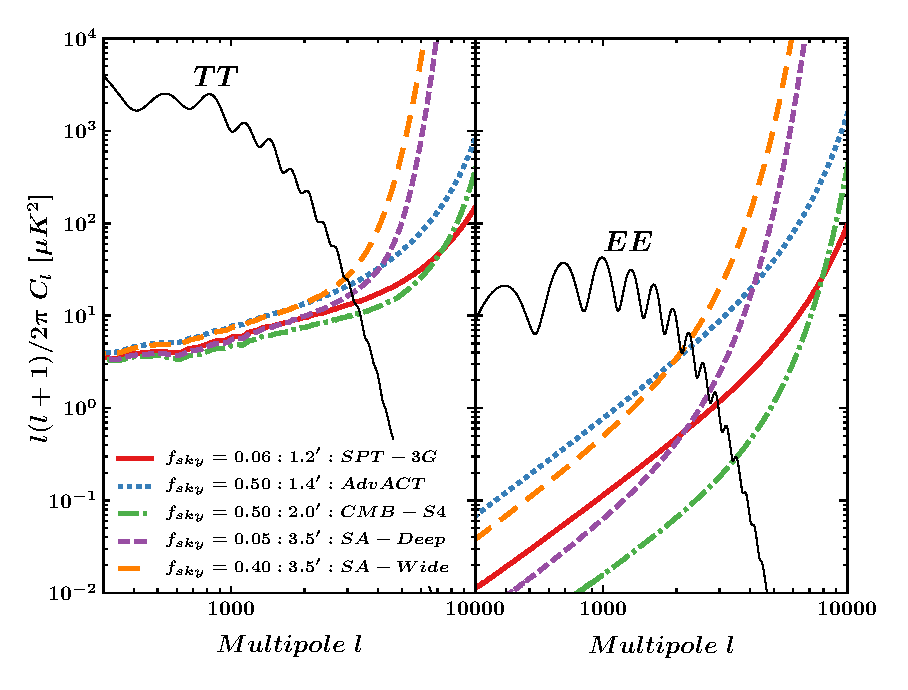
\includegraphics[width=1.\textwidth, height=0.68\textwidth,clip=]{figs/fig3.eps}
\caption{The expected residual foreground and noise power spectrum for the future CMB experiments.
The 90, 150, and 220 GHz channels have been combined using a constrained ILC technique to remove the tSZ effect while minimizing other extragalactic foregrounds and instrumental power.
The left and the right panels correspond to temperature and polarization respectively.
The plateauing of the residual temperature spectrum reflects the limited foreground removal possible with three frequency channels.
Specifications about each experiment are listed in Table \ref{tab_forecast_future_CMBexp}.}
\label{fig_ILC_res}
\end{figure}
\begin{table}[ht]
%\caption{Forecasted mass uncertainties for the future CMB experiments after foreground cleaning}
\centering
\resizebox{\columnwidth}{!}{
\begin{tabular}{|c | c | c | c | c | c | c | c | c |}
   \hline
    & \multicolumn{3}{c|}{} & \multirow{3}{*}{$f_{sky}$}& Effective & \# of &  & \\
    Experiment & \multicolumn{3}{c|}{$\Delta T$  [\ukarcmin] } & & beam & clusters & $T_{\rm ML}$ & $QU_{\rm ML}$ \\
    \cline{2-4}%\cline{7-8}
    %& { }90 & 150 &  220 & $[\theta_{_{\rm FWHM}}]$  &  & {\ \ }$T_{\rm ML}$  & $QU_{\rm ML}$ \\\hline
    & { }90 & 150 &  220 & & $[\theta_{_{\rm FWHM}}]$  & ($N_{clus}$) & (ILC)  & (ILC) \\\hline
    \multirow{3}{*}{CMB - S4} & \multirow{3}{*}{{ }1.0} & \multirow{3}{*}{{ }1.0} & \multirow{3}{*}{{ }1.0} & \multirow{3}{*}{0.50} & $1.0'$ & \multirow{3}{*}{{ }100,000} & 0.87\% & 0.83\% \\
    \cline{6-6}\cline{8-9}
    & & & &  & $2.0'$ & & 0.95\% & 0.98\% \\
    \cline{6-6}\cline{8-9}
    & & &  &  & $3.5'$ & & 1.20\% & 1.60\% \\\hline
    \hline
    SPT-3G & { }4.5 & { }2.5 & { }4.5 & 0.06 & $1.2'$ &  \multirow{4}{*}{10,000} & 3.28\% &  6.12\% \\%\hline
    \cline{1-5}\cline{6-6}\cline{8-9}
    AdvACT & { }8.0 & { }7.0 & 25.0 & 0.50 & $1.4'$ &  & 4.35\% & $>$15\% \\%\hline
    \cline{1-5}\cline{6-6}\cline{8-9}
   Simons Array - Deep & { }1.5 & { }1.5 & { }4.7 & 0.05 &\multirow{2}{*}{ $3.5'$} &  & 4.41\% & 8.45\% \\%\hline
    \cline{1-5}\cline{8-9}
   Simons Array - Wide & 5.5 & { }5.5 & 20.0 & 0.40 & &  & 5.86\% & $>$15\%\\\hline
 \end{tabular}
}
\vspace*{2mm}
%\tablecomments{
\caption{The forecasted mass uncertainties for large-aperture future CMB experiments. We combine data from 90, 150, and 220 GHz to clean the extragalactic foregrounds using a constrained ILC method designed to remove the tSZ signal while minimizing the residual foreground power and instrumental noise.  For polarization, the ILC is essentially optimal weighting of the bands for minimum noise. }
\label{tab_forecast_future_CMBexp}
\end{table}
\section{A look into the future}
\label{sec_forecast}
In this final section we forecast the cluster mass uncertainties from CMB-cluster lensing for the AdvACT , Simons Array, and SPT-3G experiments, which we will collectively refer to as the Stage III experiments, as well as the proposed CMB-S4 experiment.
In addition to presenting estimated mass uncertainties for the fiducial versions of these experiments, we examine how the mass uncertainty depends on  the beam size and map noise levels.
This information can be used to evaluate design tradeoffs while planning future experiments.

\subsection{Expected lensing mass uncertainties for future CMB experiments}
\label{sec_cmbs4}

We expect the next generation of CMB experiments, which will have substantially more detectors and a concomitant reduction in map noise levels, to dramatically improve the cluster mass calibration possible from\
 CMB-cluster lensing.
The experimental configuration of all the experiments considered is given in Table \ref{tab_forecast_future_CMBexp}.
Three options for telescope size (and therefore beam sizes) are listed for the proposed CMB-S4 experiment.
While current results have mass uncertainties of order $\ge 20$\% \citep{baxter15,madhavacheril15,placksz15}, we will show that stage III experiments to reach 3\% and CMB-S4 to approach 1\%.

There are two reasons for the improvements.
First, with more detectors comes lower map noise levels (and larger survey areas).
The deepest current experiments reach approximately $5\,\mu$K-arcmin in temperature; the Stage III surveys  (AdvACT \citep{henderson16};  Simons Array \citep{suzuki15}, and SPT-3G \citep{benson14}) forecast a few $\mu$K-arcmin; and projections for CMB-S4 are $\sim$\,1\,$\mu$K-arcmin.
Lower noise improves the lensing significance on any individual galaxy cluster.
Second, lower noise levels and larger survey areas translate into substantially more galaxy clusters.
Current ground-based SZ cluster catalogs have fewer than 1000 clusters \citep{hasselfield13, bleem15}, but SPT-3G is forecast to find 8000 clusters \citep{benson14}, AdvACT 10,000 clusters \citep{henderson16} and we assume ad-hoc that CMB-S4 will find 100,000 clusters.
In addition to the internally discovered clusters, optical surveys like DES \citep{rykoff16}, and in the future LSST \citep{lsst09} and Euclid \citep{euclid10}, will yield extremely large numbers of galaxy clusters within the CMB survey regions, as will the X-ray satellite eROSITA \citep{erosita12}.
This method is perfectly suited to determining the mass calibration for these external cluster catalogs as well.

\begin{figure*}[t]
\centering
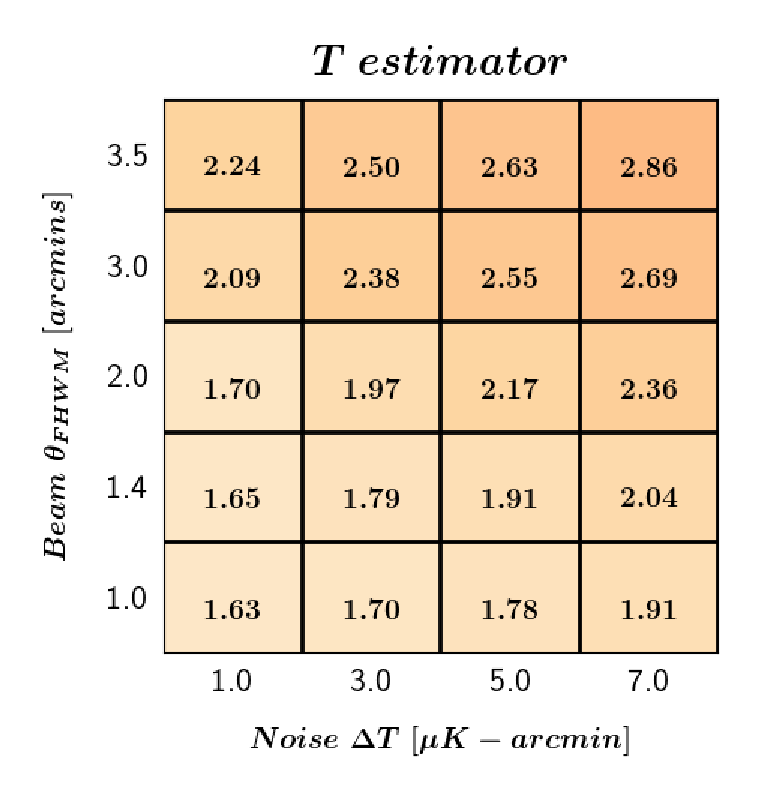
\includegraphics[width=0.46\textwidth, height=0.5\textwidth,clip=]{figs/fig4.eps}
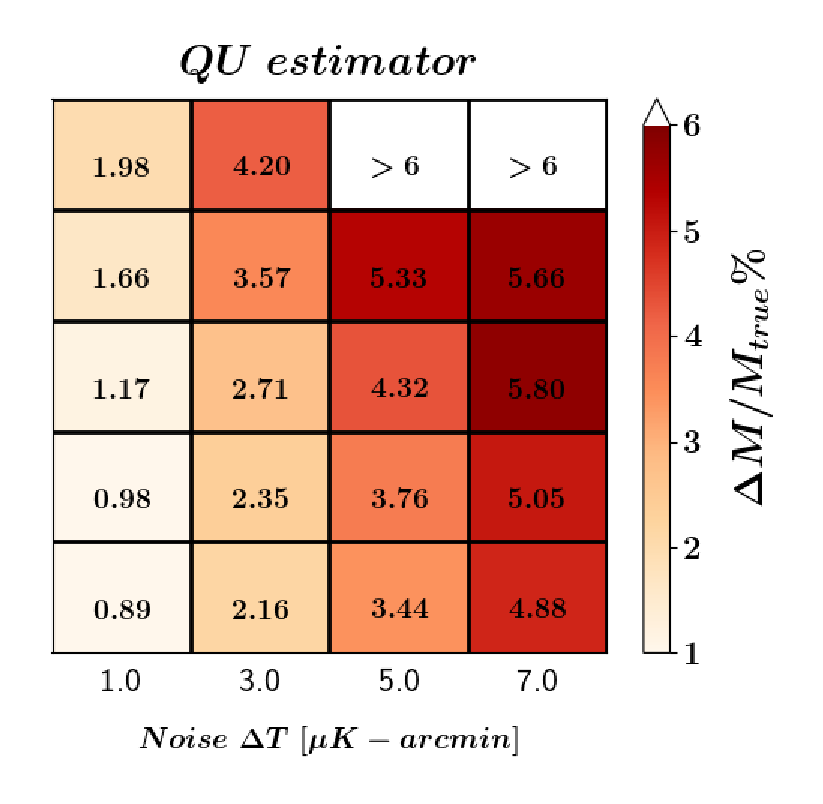
\includegraphics[width=0.5\textwidth, height=0.5\textwidth,clip=]{figs/fig5.eps}
\caption{The performance of the polarization MLE is very sensitive both to the angular resolution and map noise level of an experiment; the gains for the temperature MLE are much smaller. The numbers correspond to the CMB-cluster lensing mass uncertainty (in percent) of the cluster sample containing 100,000 clusters after the addition of foregrounds (dotted lines in right panel of Fig. \ref{fig_performance}).
Improving the beam from $3.'5$ to $1'$ enhances the SNR by a factor of two for the CMB-S4 noise levels.
The saturation of $T_{\rm ML}$ is due to the larger impact of foregrounds on the temperature maps. }
\label{fig_beam_dependency_T_QU}
\end{figure*}

To provide realistic estimates of the mass uncertainties, we perform a constrained internal linear combination (ILC) of data from 90, 150, and 220 GHz channels based on the \texttt{SMICA} (Spectral Matching Independent Component Analysis) algorithm \citep{cardoso08, planck14-09} to eliminate the tSZ signal from the temperature data and minimize the residual power in other extragalactic foregrounds and instrumental noise in both temperature and polarization.\footnote{Note that unlike in Fig~\ref{fig_performance} we consider the effect of relative beam and noise levels of different frequency channles}
The resulting power spectra of the instrumental noise and residual foregrounds for different CMB experiments are shown in Fig.~\ref{fig_ILC_res}.
At $\ell \le 2000$, the temperature curves are dominated by residual foreground power as three frequency bands are insufficient to completely eliminate the foreground power in the assumed model (see Appendix).
As a result, the temperature noise curves  converge at $\ell \le 2000$ despite the very different noise levels of the  experiments.
During this process, we convolve the 90 and 220 GHz spectra by the ratio of 150 GHz beam and their native beams, so that the final effective beam size matches 150 GHz.

The expected performance of each  experiment is given in Table \ref{tab_forecast_future_CMBexp}.
One significant uncertainty is the number of clusters to assume for each experiment.
As accurately modeling the survey selections functions for SZ, optical, and X-ray surveys is beyond the scope of this work, we make the simplifying assumption that all Stage III experiments will have 10,000 clusters and the CMB-S4 experiment will have 100,000 clusters.
This is of order the number expected to be discovered through the tSZ effect by the SPT-3G (8000 clusters; \citet{benson14}) or AdvACT (10,000 clusters; \citet{henderson16}), but likely an over-estimate for the Simons Array due to its larger 3.5$^\prime$ beam size.                                                                                                                                                      
%This is of order the number expected to be discovered through the tSZ effect by the SPT-3G or AdvACT (see above), but likely an over-estimate for the Simons Array due to its larger 3.5$^\prime$ beam size.
On the other hand, the experimental beam size is irrelevant when predicting the size of cluster samples from optical or X-ray surveys that overlap with the CMB surveys.
The DES or LSST surveys should provide samples with more than 50,000 clusters for all of the Stage III CMB experiments \citep{rykoff16, lsst09}.
Given a specific sample size, the mass uncertainty can be obtained by rescaling the numbers provided in Table \ref{tab_forecast_future_CMBexp} by $\sqrt{\frac{N_{sample}}{N_{clus}}}$.

Even considering concerns about potential biases from astrophysical signals, the temperature channel will be extremely important for the cluster mass estimates from the Stage III CMB experiments. % (AdvACT, Simons Array, SPT-3G).
 The mass uncertainty on the fiducial 10,000 cluster sample  is similar in temperature from all three experiments, with a range from 3.3\% (SPT-3G) to 5.9\% (the Simons Array wide survey). These uncertainties are as large as the likely systematic uncertainties, and the statistical uncertainties on polarization are higher by a factor of two or more. As an example of scaling the results with sample size, we replace the \
fiducial sample size by the expected number counts for SZ-discovered clusters with SPT-3G (8000) and optically detected clusters from the DES (50,000). SPT-3G would achieve a 3.6\% mass uncertainty with a sample of 8000 SZ-selected clusters and a 1.5\% uncertainty on a sample of 50,000 optically-selected clusters. The shallow portions of the Simons Array or AdvACT surveys cannot contribute much for the polarization estimator; lower noise levels are essential. The polarization estimator can be within a factor of two for the deep surveys of the Simons Array or SPT-3G. For instance, the polarization estimator for SPT-3G on 8000 clusters yields a 6.8\% mass calibration, to be compared to the 3.6\% mass calibration from temperature (ignoring systematic uncertainties).


The lower level of systematic uncertainty for polarization comes into play for the CMB-S4 experiment. First, for the extremely low noise levels of CMB-S4, the performance of the temperature and polarization channels is nearly identical (0.95\% vs.~0.98\%) for an instrument with $2'$ beam resolution. Second, the magnitude of the temperature-only systematic errors (primarily from the SZ effect) is now several times larger than the raw statistical uncertainties, and would dominate the temperature error budget. We can expect cluster mass calibrations from CMB-S4's polarization data at the 1\% level.

The mass calibration forecasts in  Table \ref{tab_forecast_future_CMBexp} are highly complementary  to and competitive with the masses obtained by stacking optical weak lensing measurements. For example, LSST hopes to achieve a mass uncertainty of 1\% by stacking few thousands of clusters at redshifts $z < 0.5$ \citep{lsst09}. At high redshifts, since the number density of background galaxies decrease rapidly, the constraints from optical lensing measurements tend to weaken. Calibrating the high redshift end of the mass function is the true power of CMB-cluster lensing which will allow us to place important constraints on the redshift evolution of mass-observable scaling relations out to high redshifts $z \ge 1.5$.

\subsection{Optimizing survey design: SNR as a function of beam size and map noise levels}
\label{sec_beam_dependence}

There are plans underway to build a substantially more sensitive CMB experiment, CMB-S4 \citep{cmbs4-sb1}, with work already underway both \
on design studies and planning for CMB-S4 and on pathfinder experiments to CMB-S4 such as the Simons Observatory. There is a wide spectrum of science drivers for these experiments, of which CMB-cluster lensing is only one. However, it is useful to consider what CMB-S4 design choices would be optimal for cluster mass calibration. In this section, we consider two lever arms: map noise levels and angular resolution (beam size). In all cases, we assume three frequency bands centered at 90, 150 and 220\,GHz with equal noise levels and beam sizes that scale as the wavelength.                                                                                                                            
We do not consider the number or relative weight of frequency bands, although these decisions will be important for handling astrophysics foregrounds in the temperature estimator.

In Fig.~\ref{fig_beam_dependency_T_QU}, we present the mass uncertainties on a sample of 100,000 clusters from the temperature and polarization estimators for a grid of five different beam sizes $\theta_{{\rm FWHM}} = 1^\prime, 1.^\prime4, 2^\prime, 3^\prime, 3.^\prime 5$, and four temperature map noise levels (1, 3, 5, or 7\,\ukarcmin{}). We have simplified the problem by using only 150\,GHz data with no foreground \
removal. As a result, the quoted uncertainties are likely to be too large for both temperature and polarization estimators.
However, the qualitative conclusions are robust to this assumption as will be shown below by spot-checking the results with a full ILC analysis.

Notably, the temperature results show only a minor improvement ($<20$\%) going from 7 to 1 \ukarcmin{} noise levels. The plateauing occurs because the instrumental noise is already smaller than the foreground power. Although the exact level may be off, these 150 GHz only results\
 are consistent with the picture from the full, 3-frequency ILC analysis shown in Fig.~\ref{fig_ILC_res}. In that figure, the residual foreground and noise power curves for temperature are essentially the same, whether from CMB-S4, from small and deep Stage III surveys, or from wide and shallow Stage III surveys. In short, foreground residual power dominates the results even at the lower sensitivities of the Stage III experiments.
The temperature estimator also shows a fairly modest effect from reducing the beam size: a factor of 3.5 reduction in beam size from $3.^\prime5$ to $1^\prime$ only improves the mass uncertainty by a factor of 1.35. This is because the foreground power floor limits the use of small-scale modes where the beam size matters most.

In contrast, as seen in the right panel of Fig.~\ref{fig_beam_dependency_T_QU}, the fidelity with which the QU polarization estimator recovers cluster masses is strongly dependent on the experimental noise level and beam size. The clear improvements are because polarization estimator is still noise instead of residual foreground dominated. Improving map noise levels from 3 to 1 \ukarcmin{} improves the SNR on CMB-cluster lensing by a factor of 2.4 (the equivalent change for the temperature estimator is only 1.04). Similarly, reducing the beam size three\
fold from $3^\prime$ to $1^\prime$ leads to an improvement by a factor of 1.9. Both the beam size and instrumental noise levels matter for the performance of the polarized CMB-cluster lensing estimator.

Finally, we confirm this picture by extending these 150\,GHz-only predictions to 3-band data using the ILC method. We assume equal temperature map noise levels of $1 \mu$K-arcmin at 90, 150 and 220\,GHz, with a beam size that scales with the wavelength. We consider three 150\,GHz\
 beam sizes, $1^\prime, 2^\prime$, and $3.^\prime 5$, with the results  tabulated in Table~\ref{tab_forecast_future_CMBexp}.
The improvement  as a function of the beam size is consistent between the 150\,GHz and ILC cases. While the improvement is only marginal for\
 the temperature channel, the mass uncertainty from the polarization estimator drops to 0.83\% for a $1^\prime$ beam, a factor of 1.9 better\
 than the results for a $3.^\prime5$ beam. The corresponding improvement for 150\,GHz only is slightly better, at a factor of 2.2.
 
 \section{Conclusion}
\label{sec_conclusion}
We have developed MLEs to optimally extract lensing information from the temperature (T) and polarization (Q/U) maps of the CMB. We show a Q/U based MLE recovers as much information as an estimator using E and B mode maps. We also show that the temperature MLE performs better than the standard QE by a factor of two at very low noise levels in the absence of astrophysical foregrounds; the performance gain is not significant for the polarization estimator due to the lower SNR. We consider the effects of these foregrounds on the cluster lensing estimators,\
 finding at 150\,GHz that  astrophysical foregrounds have no impact on the polarization MLE and set an effective noise floor of a few \ukarcmin{} on the temperature MLE unless removed using multi-frequency data.

We quantify the systematic uncertainties due to astrophysical foregrounds (the tSZ effect, kSZ effect or dusty galaxies), uncertainty in the\
 cluster position or redshift, projection effects from nearby lower-mass haloes, and uncertainty in the cluster mass profile. We find that the dusty galaxies in the cluster are likely to bias the temperature(polarisation) MLE at -4.5\%(-1.3\%) level.  The biases due to uncertainty in the cluster position or redshift are manageable for both temperature and polarization. Lower mass haloes near the galaxy cluster lead to an overestimate of the cluster masses at the 2.5 to 6.3\% level, and will need to be carefully accounted for using simulations.
The uncertainties in the cluster mass profile can shift the cluster mass either up or down by up to a few percent. Better measurements of the cluster mass profile are needed to reduce this uncertainty.

The clusters own SZ signals induce significant bias on temperature MLE. The kSZ effect has the same spectral dependance as that of CMB and cannot be removed using multiple frequency channels; it will induce a bias of -7.3\% on temperature MLE. tSZ induce significant biases on MLE estimators if not taken into account. tSZ is an order of magnitude greater than lensing signal and if not taken into account will kill the lensing signal. We can exploit multiple frequency channels to remove tSZ, however, that will decrease the SNR by a factor of three \citep{baxter15}. In the next two chapter we will introduce modified QE to eliminate the tSZ bias with negligible decrease in SNR. 

Finally, we present forecasts for the mass uncertainties from upcoming CMB experiments,  combining multiple frequency bands with an ILC technique to minimize the instrumental noise and astrophysical foregrounds. The AdvACT, Simons Array and SPT-3G experiments will achieve mass calibration uncertainties of order 3 - 6\% for a sample containing 10,000 clusters, with the temperature channel being crucial to these mass constraints. With the even lower noise levels of CMB-S4 and a $2^\prime$ beam, we find the statistical mass uncertainty from either the temperature or polarization MLEs falls to just below 1\% with 100,000 clusters. We expect polarization to be the main information channel for CMB-S4 given the potential biases  due to the temperature foregrounds. Finally, we consider how the performance of CMB-S4 depends on the assumed noise level or beam size, finding that a factor of three reduction in either the beam size or noise level leads to roughly a factor of two improvement on the mass calibration from the polarization MLE. CMB-S4 has the potential to transform galaxy cluster cosmology by reducing the current 20\% mass uncertainty on galaxy clusters twentyfold to $\sim$\,1\%.



